% !TEX root = relatorio.tex
%
% Capítulo 4 — Arquitetura e Fundações
%
\chapter{Arquitetura e Fundações} \label{cap:desenvolvimento}

\section{Arquitetura Geral do Sistema} \label{sec:arquitetura}

O Play4Change está estruturado em torno de uma ideia simples: quem consome a plataforma nunca fala diretamente com quem gera, guarda ou protege o que é consumido. O Administrador cria e gere conteúdo através do cliente web; o Learner consome-o através do desafio diário no cliente móvel (RF07). Entre os dois e o resto do sistema fica sempre um núcleo que decide o que fazer, sem depender de como cada peça está concretizada. A Figura~\ref{fig:arquitetura} apresenta essa estrutura.

\begin{figure}[h!]
    \centering
    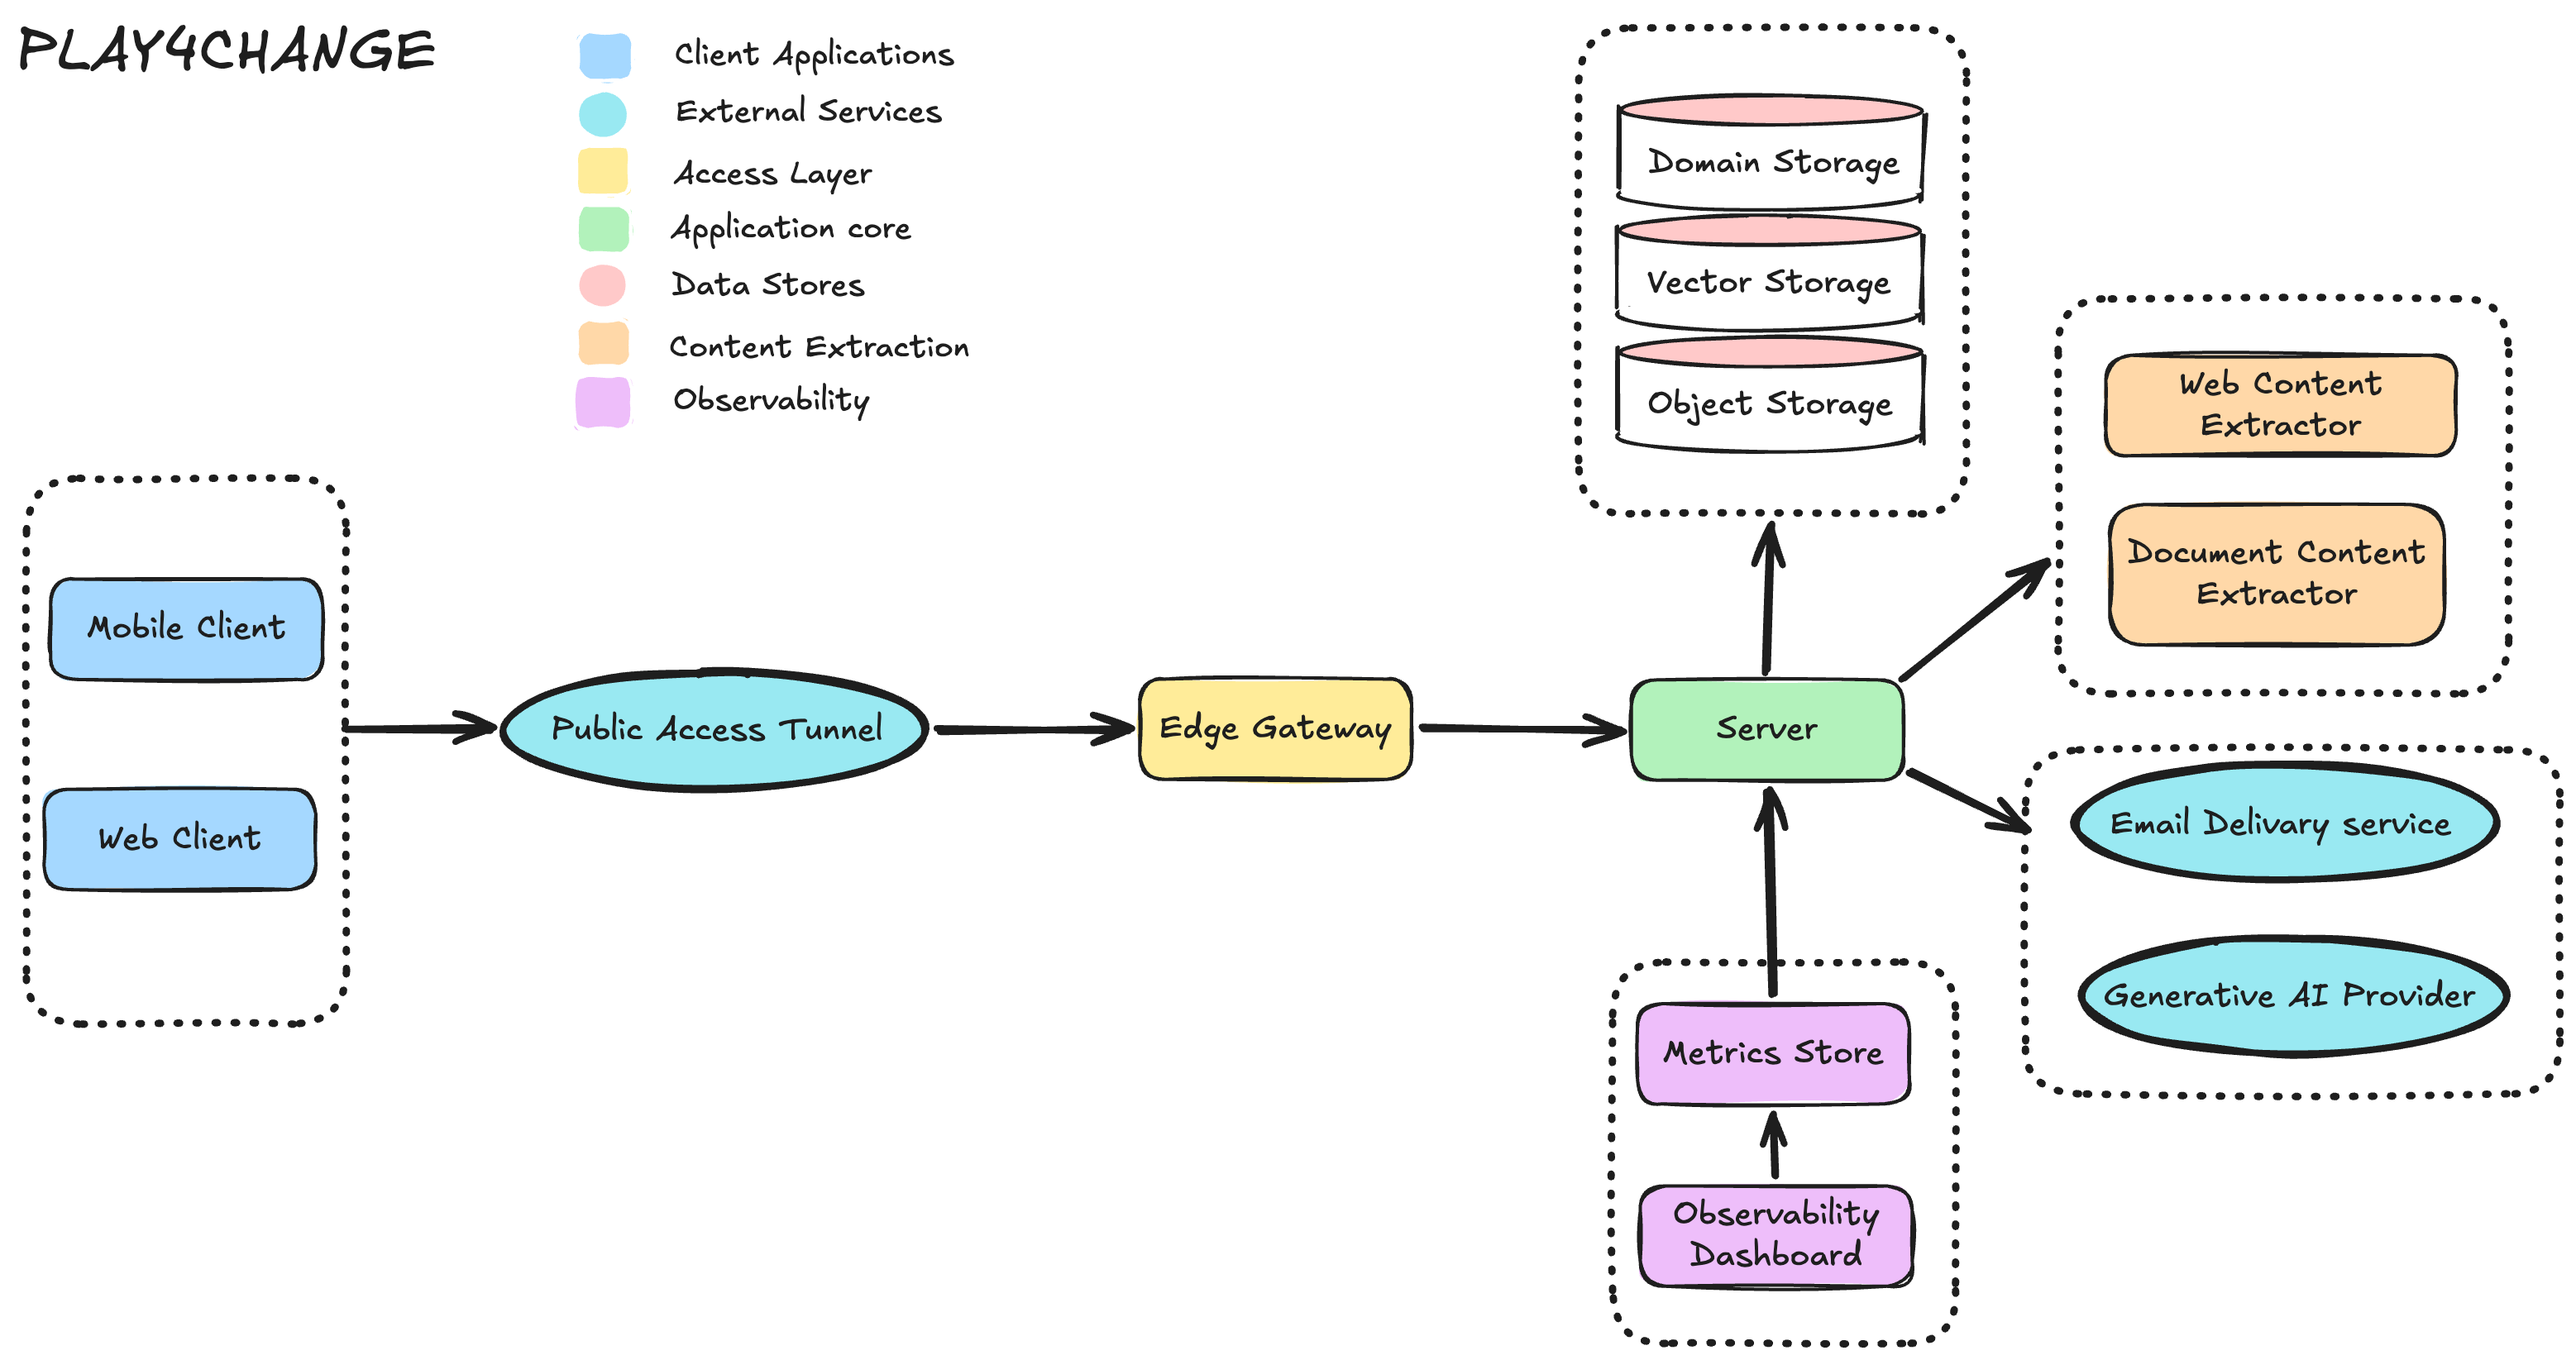
\includegraphics[width=\textwidth]{./figures/Architecture-p4c.png}
    \caption{Arquitetura geral do sistema Play4Change}
    \label{fig:arquitetura}
\end{figure}

Os dois clientes entram pelo mesmo caminho: um túnel de acesso público, que assegura que o tráfego dos clientes não expõe uma porta diretamente e que essa comunicação é cifrada (RNF01), seguido por uma cadeia de filtros de borda que filtra e autentica (RF01) antes de qualquer pedido chegar à lógica de negócio.

Só depois de atravessar este perímetro é que um pedido chega ao núcleo. É o núcleo que resolve o desafio diário do Learner, adapta o percurso quando há dificuldade e escala para tutoria quando a adaptação não é suficiente (RF04--RF06); e que, do lado do Administrador, recebe um documento ou URL e decide gerar tópicos e desafios a partir dele (RF02, CU01).

Para isso, o núcleo depende de quatro tipos de capacidade externa, e nunca fala diretamente com nenhuma implementação concreta de nenhuma delas, apenas com o que cada uma promete fazer: extrair conteúdo de uma fonte, gerar conteúdo pedagógico e explicações, persistir e indexar semanticamente o que já foi gerado para o reutilizar sempre que possível (RF03), e notificar o utilizador. O sistema é ainda observado de fora: métricas de funcionamento são recolhidas periodicamente a partir do núcleo, sem que essa recolha interfira com nenhum pedido em curso.

Esta indireção não é um detalhe acidental: é o que garante que trocar qualquer uma destas capacidades por outra equivalente não obriga a tocar na lógica de negócio (RNF04), e é o que torna o núcleo testável isoladamente, sem depender de nenhuma delas estar de facto disponível.

Um pedido típico atravessa este perímetro antes de chegar à lógica de negócio; o Capítulo~\ref{cap:implementacao} detalha, já ao nível de implementação, como cada uma destas fronteiras foi concretizada.
